\chapter{Espaces préhilbertiens ou euclidiens}
\labch{espaces_prehilbertiens_ou_euclidiens}

Lorsque $E$ est un espace euclidien, le procédé de \textsc{Gram}-\textsc{Schmidt} permet, à partir d'une base adaptée à un drapeau total de $E$, d'obtenir une base orthonormale adaptée à ce même drapeau. \\
Si l'on combine avec le théorème de trigonalisation utilisant les drapeaux, on constate que tout endomorphisme trigonalisable peut être trigonalisé dans une base orthonormale. 

\marginnote[-3cm]{
    \begin{kaobox}[frametitle=Drapeau]
        (Wiki) \\
        Un \emph{drapeau} d'un espace vectoriel $E$ de dimension finie est une suite finie strictement croissante de sous-espaces vectoriels de $E$, commençant par l'espace nul $\{0_E\}$ et se terminant par l'espace total $E$:
        $$\{0_E\} = E_0 \subsetneq E_1 \subsetneq \cdots \subsetneq E_k = E.$$
        Si $\dim(E)=n$ et si pour tout $i \in \llbracket 1, k \rrbracket$, $\dim(E_i)=i$, alors le drapeau est dit \emph{total}.
    \end{kaobox}
}

\newpage

\section{Déterminant de \textsc{Gram}} \label{matrice_gram}
\begin{tcolorbox}
    Soit $E$ un espace euclidien et $(x_1, \dots, x_p)$ une famille d'éléments de $E$. On définit
    $$\text{la matrice de \textsc{Gram} } \Gram = \left( \langle x_i, x_j \rangle \right)_{i,j \in \llbracket 1, p \rrbracket}$$
    $$\text{le déterminant de \textsc{Gram} } \Gram(x_1, \dots, x_p) = \det \Gram.$$
    On remarque que $\Gram$ est symétrique. 
    Le déterminant de \textsc{Gram} permet de calculer des volumes et de tester l'indépendance linéaire d'une famille de vecteurs.
\end{tcolorbox}

Résultats: à compléter à partir de \url{https://fr.wikipedia.org/wiki/Déterminant_de_Gram}
\begin{itemize}
    \item La matrice de \textsc{Gram} est toujours positive.
    \item La famille $(x_1, \dots, x_p)$ et sa matrice de \textsc{Gram} ont le même rang.
    \item La famille $(x_1, \dots, x_p)$ est liée si et seulement si $\det \Gram(x_1, \dots, x_p) = 0$.
    \item Soit $F = \Vect(x_1, \dots, x_p)$,
    $$\forall x \in E,\ \det \Gram(x, x_1, \dots, x_p) = d^2(x, F) \times \det \Gram(x_1, \dots, x_p)$$
\end{itemize} 

\begin{enumerate}
    \item Montrer que la famille $(x_1, \dots, x_p)$ est liée si et seulement si $\Gram(x_1, \dots, x_p) = 0$. \\
    $(\Rightarrow)$ Il existe une famille $(\lambda_1, \dots, \lambda_p)$ non nulle  de $\R^n$ telle que $\sum\limits_{i=1}^{p} \lambda_i x_i = 0$. On montre alors que pour tout ligne $L_i$ de $\Gram$, $\sum\limits_{i=1}^{p} \lambda_i L_i = 0$ ce qui permet de conclure. \\
    $(\Leftarrow)$ Raisonner par contraposée, on suppose $\mathscr{F}$ libre. \\
    Soit $\mathscr{B} = (\varepsilon_1, \dots, \varepsilon_n)$ une b.o.n. de $E$ et $H \in \M_{n, p} (\R)$ la matrice de $\mathscr{F} = (x_1, \dots, x_p)$ dans $\mathscr{B}$. \\
    Alors $\boxed{\Trsp{H} H = G(x_1, \dots, x_p)}$. \\
    Montrons la chaîne :
    $$\Rg(G) = \underbrace{\Rg(\Trsp{H} H) = \Rg(H)}_{\text{à montrer}} = \Rg(\mathscr{F}) = p \not= 0$$
    Montrer que $\Rg(\Trsp{H} H) = \Rg(H)$ en montrant que $\Ker(\Trsp{H} H) = \Ker(H)$. 
    \begin{itemize}
        \item $(\subset)$ oui
        \item $(\supset)$ Soit $X \in \Ker(\Trsp{H}H)$. On montre que $\norme{BX} = 0 \Rightarrow BX = 0$. 
    \end{itemize}
    Par le \textbf{théorème du rang}, on obtient le résultat. 
\end{enumerate}

\begin{tcolorbox}
    La matrice de \textsc{Gram} est symétrique positive.
\end{tcolorbox}

\begin{proof} \\

    \begin{itemize}
        \item La matrice de \textsc{Gram} est symétrique par symétrie du produit scalaire.
        \item Montrons la positivité de $\Gram$. Soit $X = \Trsp{(\alpha_1 \cdots \alpha_n)} \in \M_{n,1}(\R)$. Montrons que $\Trsp{X} \Gram X \geqslant 0$. 
        \begin{align*}
            \Trsp{X} \Gram X &= \sum_{i=1}^{n} \sum_{j=1}^{n} \langle x_i, x_j \rangle \alpha_i \alpha_j \\ 
            &= \sum_{i=1}^{n} \sum_{j=1}^{n} \langle \alpha_i x_i, \alpha_j x_j \rangle \\
            &= \left\Vert \sum_{i=1}^{n}x_i \alpha_i \right\Vert^2 \geqslant 0.
        \end{align*}
    \end{itemize}
   
    Ce qui montre bien que $\Gram$ est symétrique positive.
\end{proof}

\marginnote[-4cm]{
    \begin{kaobox}[frametitle=Matrices symétriques positives]
        L'ensemble des \emph{matrices symétriques positives} est noté $\mathscr{S}_n^+(\R)$. Une matrice $M \in \mathscr{S}_n^+(\R)$ équivaut à chacune des propriétés suivantes:
        \begin{itemize}
            \item pour tout $X \in \M_n(\R), \Trsp{X} M X \geqslant 0$,
            \item $\Sp(M) \subset \Rp.$
        \end{itemize}
    \end{kaobox}
}


\section{Positivité de la matrice de \textsc{Hilbert}}
\marginnote[0cm]{(Planche n°14. Espaces euclidiens de \cite{maths-france})}
Si on interprète le terme général de la matrice de \textsc{Hilbert} (cf. \nameref{matrice_hilbert}) comme 
$$\Hilb_{i,j} = \int_{0}^{1} x^{i+j-2} \d x$$
on peut y reconnaître une \nameref{matrice_gram} pour les fonctions puissances et le produit scalaire usuel sur l'espace des fonctions de $[0, 1]$ dans $\R$ de carré intégrable. Puisque les fonctions puissances sont linéairement indépendantes, les matrices de \textsc{Hilbert} sont donc
\href{https://fr.wikipedia.org/wiki/Matrice_de_Hilbert}{définies positives}.


\section{Décompositions matricielles}
Voir le thème 23 de \cite{acamanes}.
\subsection{Décomposition d'\textsc{Iwasama}}
\begin{prop}
    Soient $n \in \Ne$ et $M \in \Gl_n(\R)$. Il existe un \textbf{unique} couple $(T, O)$ tel que:
    $$M = OT,$$
    avec $T$ triangulaire supérieure à coefficients diagonaux strictement positifs et $O$ matrice orthogonale. 
\end{prop}

Comme $M$ est inversible, c'est une matrice de changement de base. \\
Le produit et l'inversibilité sont stables dans $\mathscr{T}_n^+$.

\marginnote[-2cm]{
    \begin{kaobox}[frametitle=Le procédé de \textsc{Gram}-\textsc{Schmidt}]
        Soit $E$ un espace vectoriel préhilbertien et soit $\mathscr{F} = (e_i)_{i \in I}$ une famille libre dans $E$; il existe une unique famille orthonormale $\mathscr{G} = (\varepsilon_i)_{i \in I}$ telle que pour tout $k \in \llbracket 1, n \rrbracket$,
        \begin{itemize}
            \item $\Vect(e_1, \dots, e_k) = \Vect(\varepsilon_1, \dots, \varepsilon_k)$,
            \item $\langle e_k, \varepsilon_k \rangle > 0$.
        \end{itemize}
        La famille $\mathscr{G}$ est appelée l'\emph{orthonormalisée (de \textsc{Gram}-\textsc{Schmidt})} de $\mathscr{F}$.
    \end{kaobox}
}

\begin{preuve}
    \begin{itemize}
        \item \underline{Existence:} \\
        On note $\mathscr{B}$ la base canonique de $\R^n$. Soit $\mathscr{C} \defeq (C_1, \dots, C_n)$ la famille des vecteurs colonnes de $M$ exprimés dans $\mathscr{B}$. Comme $M$ est inversible, $\mathscr{C}$ forme une \textbf{base} de $\R^n$. Appliquons-lui le \textbf{procédé d'orthonormalisation de \textsc{Gram}-\textsc{Schmidt}}. \\
        Il existe une base orthonormée $\mathscr{B}_O = (O_1, \dots, O_n)$ telle que pour tout $i \in \llbracket 1, n \rrbracket$
        $$\mathrm{Vect}(C_1, \dots, C_i) = \mathrm{Vect}(O_1,\dots, O_i) \quad (1) \quad \text{et} \quad \langle C_i, O_i \rangle > 0 \quad (2).$$
        On écrit $M = P_{\mathscr{B} \to \mathscr{C}} = P_{\mathscr{B} \to \mathscr{B}_O} \times P_{\mathscr{B}_O \to \mathscr{C}} = OT$. \\
        Le caractère triangulaire de $T = P_{\mathscr{B}_O \to \mathscr{C}}$ vient de $(1)$ et la stricte positivité de sa diagonale de $(2)$.
        \item \underline{Unicité:} \textcolor{green}{à compléter} \\
        Soit $M = OT = O'T'$. $T$ est inversible. $(O')^{-1}O =T'\Inv{T}$. Le premier terme est une matrice orthogonale et le second triangulaire supérieure car ces deux ensembles sont des groupes multiplicatifs. $B = T'\Inv{T}$ est diagonale (schéma) de coeff...
    \end{itemize} 
\end{preuve}

\subsection{Décomposition polaire d'une matrice}
Lire chapitre 7 de \cite{matrices} page 77.

\section{Inégalité d'\textsc{Hadamard}}
%\begin{marginfigure}[-1cm]
%    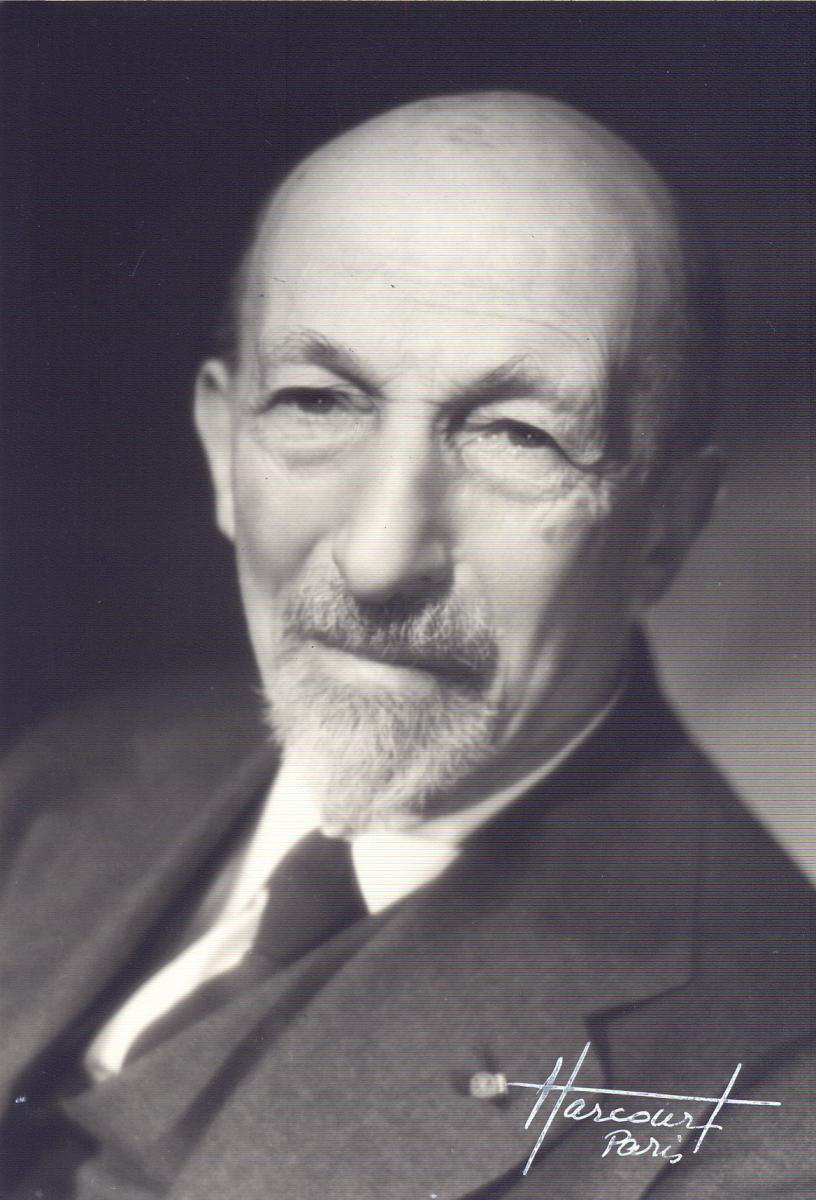
\includegraphics[width=5cm]{images/jacques_hadamard.jpg}
%    \caption{Jacques \textsc{Hadamard}}
%\end{marginfigure}

\begin{theo}{Inégalité d'\textsc{Hadamard}}
    Soit $M \in \M_n(\C)$ et soient $X_1, \dots, X_n$ ses vecteurs colonnes. Alors,
    $$|\mathrm{det} M | \leqslant \prod_{i=1}^{n} \Vert X_i \Vert$$
    avec égalité si et seulement si la famille $(X_i)_{1 \leqslant i \leqslant n}$ est orthogonale.
\end{theo}

%\begin{marginfigure}[-2cm]
%    \resizebox{6.5cm}{6.5cm}{%
    \begin{tikzpicture}
        \node[block] (gram) {Déterminant \\ de \textsc{Gram}};
        \node[block, right of=s1] (iwasama) {Décomposition \\ d'\textsc{Iwasama}};
        \node[block, below right of=gram] (hadamard) {Inégalité \\ d'\textsc{Hadamard}};
    
        \draw (gram) edge[bend right, above left] node {...} (hadamard);
    
        \draw (iwasama) edge[bend left] node {$M=OT$} (hadamard);
    
    \end{tikzpicture}    
}
%\end{marginfigure}

Voyons deux démonstrations de ce résultat; une première en utilisant la décomposition d'\textsc{Iwasama} et une deuxième le \refthm{inegalite_gram}.

\begin{preuve}
    \begin{itemize}
        \item Si la matrice $M$ n'est pas inversible alors $\det M = 0$ et comme une norme est à valeurs positives, le résultat est immédiat. 
        \item Supposons que $M$ est inversible. D'après la décomposition d'\textsc{Iwasama}, il existe une matrice $O \in \mathscr{O}_n(\C)$ et $T \defeq (t_{i,j})_{1 \leqslant i, j \leqslant n}$, triangulaire supérieure dont les coefficients diagonaux sont strictement positifs telles que $M = OT$. D'après la multiplicité du déterminant, 
        $$\det M = \det(O) \det(T).$$
        Or $\det O = \pm 1$ donc
        \begin{equation} \label{det}
            |\det M | = |\det T | = \prod_{i=1}^{n} |t_{i,i}|.
        \end{equation}
        Par construction, pour tout $i \in \llbracket 1, n \rrbracket, t_{i,i} \defeq \langle X_i, O_i \rangle$ où $O_i$ est un vecteur unitaire. D'après l'inégalité de \textsc{Cauchy}-\textsc{Schwarz}, pour tout $i \in \llbracket 1, n \rrbracket$, 
        $$|t_{i,i}| = |\langle X_i, O_i \rangle | \leqslant \norme{X_i} \underbrace{\norme{O_i}}_{=1}.$$
        Ainsi d'après (\ref{det}), 
        $$|\det(M)| \leqslant \prod_{i=1}^n \norme{X_i}.$$
    \end{itemize}
        \textcolor{red}{cas d'égalité}
\end{preuve}

\begin{preuve}
    \begin{itemize}
        \item Si la matrice $M$ n'est pas inversible, le résultat est immédiat. 
        \item Supposons que $M$ est inversible. On a 
        $$\Trsp{M} M = \Gram(X_1, \dots, X_n),$$ 
        la matrice de \textsc{Gram} de la famille des colonnes de la matrice $M$. 
        En composant cette relation par le déterminant, 
        $$\det(\Trsp{M}M) = \det \big( \Gram(X_1, \dots, X_n) \big) = \det(M)^2 $$
        car $\det(\Trsp{M}) = \det M$.
        D'après le (\ref{inegalite_gram}), 
        \begin{align*}
            \det \Gram(X_1, \dots, X_n) &\leqslant \prod_{i=1}^n \norme{X_i}^2 \\
            \text{soit } \det (M)^2 &\leqslant \prod_{i=1}^n \norme{X_i}^2
        \end{align*}
        En passant à la racine on obtient l'inégalité d'\textsc{Hadamard}.
    \end{itemize}
\end{preuve}

\marginnote[0cm]{
    \begin{kaobox}[frametitle=Parallélotope]
        Soit $(x_1, \dots, x_n)$ une famille libre. Le parallélotope engendré par cette famille est défini par
        $$P \defeq \left\{ x = \sum_{i=1}^n t_i x_i,\ \forall i\ t_i \in [0,1]\right\}.$$
    \end{kaobox}
}

L'inégalité d'\textsc{Hadamard} nous apprend que le volume du parallélotope défini par les vecteurs colonnes est inférieur ou égal au produit des normes de ses vecteurs et il y a égalité si et seulement si la matrice est diagonale, ou encore que le parallélotope est rectangle. 

\begin{prop}{}
    Soient $\mathscr{S}_n ^{++} (\R)$ l'ensemble des matrices réelles d'ordre $n$ symétriques à valeurs propres strictement positives et $A = (a_{i,j}) \in \mathscr{S}_n ^{++} (\R)$. Alors,
    $$\det(A) \leqslant \prod_{i=1}^{n} a_{i,i}.$$
\end{prop}

\begin{exercice}    
\marginnote[0cm]{exercice 4, TD 14 \cite{acamanes}}
\begin{enumerate}
    \item Soit $(\gamma_1, \dots, \gamma_n) \in (\Re)^n$. Montrer que $B = (\gamma_i \gamma_j a_{i,j}) \in \mathscr{S}_n^{++}(\R)$. 
    \item Montrer que $\det(A)^{1/n} \leqslant \frac{\Tr(A)}{n}$. \\
    \emph{On pourra utiliser l'inégalité arithmético-géométrique}.
    
    \marginnote[-2cm]{
    	\begin{kaobox}[frametitle=Inégalité arithmético-géométrique]
            Soient $n \in \Ne$ et $x_1, \dots, x_n$ des réels positifs. Alors, 
            $$\frac{x_1 + \cdots + x_n}{n} \geqslant \sqrt[n]{x_1 \cdots x_n}.$$
            Il y a égalité si et seulement si tous les $x_i$ sont égaux.
        \end{kaobox}
        Pour d'autres inégalités, lire le chapitre 16, p.117 de la deuxième édition de Raisonnements divins (en fr)
    }
    \item Montrer que pour tout $i \in \llbracket 1, n \rrbracket, a_{i,i} > 0$. On pose $\gamma_i = \frac{1}{\sqrt{a_{i,i}}}$. En déduire l'inégalité d'\textsc{Hadamard}.
\end{enumerate}
\end{exercice}


\section{Familles de polynômes orthogonaux}
Soient $I$ un intervalle non vide de $\R$ et $w \in \mathscr{C}(I, \Rpe)$. On suppose que, pour tout entier naturel $n$, $\int_I |x|^n w(x) \d x$ converge. On note
$$\mathscr{H} \defeq \ens[\Bigg]{ f \in \mathscr{C}(I, \R) \tq \int_I f^2 w \text{ converge}}.$$
Pour tout $(P, Q) \in \R[X]^2$, on pose 
$$\langle P, Q \rangle \defeq \int_I P(t) Q(t) w(t) \d t.$$

\subsection{Construction}

\begin{exercice}
    \marginnote[0cm]{Source : \cite{acamanes} \href{https://acamanes.github.io/psi/psi_doc/chap_e13.pdf}{(Exercice 17 Ch 13)}}
    \begin{enumerate}
        \item Montrer que $\langle \cdot, \cdot \rangle$ est un produit scalaire sur $\R[X]$.
        \item Montrer qu'il existe une suite $(P_n)_{n \in \N}$ de polynômes tels que 
        \begin{itemize}
            \item pour tout $n \in \N, \deg P_n = n$,
            \item pour tout $(n, m) \in \N^2, n \not= m, \langle P_n, P_m \rangle = 0$,
            \item pour tout $n \in \N$, $P_n$ est unitaire.
        \end{itemize}
        Soit $n$ un entier naturel.
        \item Montrer que $\Vect(P_0, \dots, P_n) = \R_n[X]$.
        \item Montrer que $P_{n+1} \in \R_n[X]^\perp$.
    \end{enumerate}
\end{exercice}

\begin{solution}
    \marginnote[0cm]{Source : Solution de \cite{acamanes}}
    \begin{enumerate}
        \item 
        \begin{itemize}
            \item[$\rhd$] Montrons que $\langle \cdot, \cdot \rangle$ est bien définie. D'une part, $PQw$ est une fonction continue sur $I$. \\
            De plus, $|PQ| \leqslant \frac{P^2 + Q^2}{2}$. Comme $w$ est à valeurs positives, alors
            $$|PQw| \leqslant \frac{1}{2} \Big[ P^2 w + Q^2 w\Big].$$
            Comme $P^2 w$ et $Q^2 w$ sont intégrables sur $I$, d'après les théorèmes de comparaison, $PQw$ est intégrable sur $I$.
            \item[$\rhd$] $\langle \cdot, \cdot \rangle$ est bien symétrique par commutativité du produit de deux polynômes. 
            \item[$\rhd$] est bilinéaire par linéarité des intégrales convergentes.
            \item[$\rhd$] Soit $P \in \R_n[X]$. Comme $w \geqslant 0$, par croissance de l'intégrale, 
            $$\int_I P(x)^2 w(x) \d x \geqslant 0.$$
            De plus, si $\displaystyle \int_I P^2 w = 0$, comme $P$ est une fonction polynomiale donc continue et $w$ est continue, d'après la positivité de l'intégrale,
            $$\forall t \in I, P(t)^2 w(t) = 0.$$
            De plus, $w$ est à valeurs strictement positives, donc
            $$\forall t \in I, P(t) = 0.$$
            Ainsi, $P$ possède une infinité de racines distinctes et $P$ est le polynôme nul.
        \end{itemize}
        Finalement, $\langle \cdot, \cdot \rangle$ est une forme bilinéaire définie positive, donc elle définit un produit scalaire. 
        \item La famille $(X^n)_{n \in \N}$ est la base canonique de $\R[X]$. En appliquant le procédé d'orthogonalisation de \textsc{Gram}-\textsc{Schmidt} à cette famille, on construit une famille de polynôme $(P_n)_{n \in \N}$ telle que, pour tout $n \in \N$, il existe $(\lambda_0, \dots, \lambda_{n-1}) \in \R^n$ tel que
        $$P_n \defeq X^n + \sum_{j=0}^{n-1} \lambda_j P_j.$$
        Ainsi, pour tout $n \in \N$, $\deg P_n = n$ et $P_n$ est unitaire. \\
        De plus, $(P_n)_{n \in \N}$ est une famille orthogonale et 
        $$\forall (m, n) \in \N^2, m \not= n, \langle P_n, P_m \rangle = 0.$$
        \item D'après le procédé de \textsc{Gram}-\textsc{Schmidt}, pour tout $n \in \N$,
        \begin{align*}
            \Vect(P_0, \dots, P_n) &= \Vect(1, X, \dots, X^n)\\
            &= \R_n[X].
        \end{align*}
        \item Soit $P \in \R_n[X]$. D'après la question précédente, il existe $(\mu_0, \dots, \mu_n) \in \R^{n+1}$ tel que
        $$P = \sum_{k=0}^n \mu_k P_k.$$
        Alors, par linéarité du produit scalaire,
        \begin{align*}
            \langle P_{n+1}, P \rangle &= \sum_{k=0}^n \mu_k \langle P_k, P_{n+1} \rangle \\
            &= 0.
        \end{align*}
        Ainsi, $P_{n+1} \in \R_n[X]^\perp$.
    \end{enumerate}
\end{solution}

\subsection{Racines}

\begin{exercice}
    On note $(\alpha_i)_{i \leqslant i \leqslant k}$ les racines de $P_n$ qui appartiennent à $\mathring{I}$ et qui sont de multiplicité impaire. On pose $Q \defeq \prod\limits_{i=1}^k (X - \alpha_i)$.
    \begin{enumerate}
        \item Majorer le degré de $Q$.
        \item Déterminer le signe de $P_n Q$ sur $I$.
        \item En déduire que $k = n$ et que $P_n$ a toutes ses racines réelles et simples dans $\mathring{I}$.
    \end{enumerate}
\end{exercice}

\begin{solution}
    Nous allons montrer que $P_n$ admet au moins $n$ changements de signe dans $I$. C'est pour cela que nous considérons les racines de multiplicité impaire, ce sont elles qui correspondent aux changements de signe. 
    \begin{enumerate}
        \item Comme $\deg P_n = n$, le polynôme $P_n$ possède au plus $n$ racines réelles distinctes. Ainsi, $\deg Q \leqslant n$.
        \item En notant $a_1, \dots, a_p$ les racines réelles distinctes de $P$, on écrit sous forme irréductible:
        $$P_n = \prod_{i=1}^p (X - a_i)^{r_i} \prod_{i=1}^s (X^2 + b_i X + c_i)^{\ell_i}.$$
        Ainsi, pour tout $i \in \llbracket 1,p \rrbracket$, il existe $d_i \in \R$ non nul tel que
        $$P_n(x) \isEquivTo{a_i} d_i (x - a_i)^{r_i}.$$
        Alors, pour tout $i \in \llbracket 1, k$, il existe $\tilde{d_i} \in \R$ non nul tel que
        $$P_n(x) Q(x) \isEquivTo{\alpha_i} \tilde{d_i} (x - \alpha_i)^{r_i+1}.$$
        Comme $r_i$ est impair, le polynôme $P_nQ$ ne change pas de signe au voisinage de $\alpha_i$. \\
        De plus, si $a_i$ est une racine de $P_n$ de multiplicité paire, alors $P_n$ ne change pas de signe au voisinage de $a_i$, d'après la \textcolor{red}{première} question. \\
        Finalement, $P_nQ$ garde un signe constant sur $I$.
        \item Supposons par l'absurde que $k < n$.  Alors, $Q \in \R_k[X] \subset \R_{n-1}[X]$ et, d'après la question $4.$, $P_n \in \R_{n-1}[X]^\perp$. Alors,
        \begin{align*}
            \langle P_n, Q \rangle &= 0 \\
            \int_I P_n(t) Q(t) w(t) \d t &= 0.
        \end{align*}
        D'après la question précédente, $P_n Q w$ est une fonction continue et de signe constant. Ainsi, d'après la positivité de l'intégrale, $P_n Q w = 0$ sur $I$. Comme $w$ est à valeurs strictement positives,
        $$\forall x \in I, P_n(x) Q(x) = 0.$$
        Ainsi, $P_n Q$ possède une infinité de racines soit $P_n Q = 0$. Or $Q \not= 0$, soit $P_n = 0$, ce qui est absurde. Finalement, $k=n$ \note \marginnote[0cm]{\note $P_n$ a au moins $n$ changements de signe sur $I$; par le théorème des valeurs intermédiaires, $P_n$ a au moins $n$ racines dans $I$ et comme $P_n$ est de degré $n$, il y a exactement $n$ racines simples.} et $\deg Q = n$, donc toutes les racines de $P_n$ sont simples et appartiennent à $\mathring{I}$. 
    \end{enumerate}
\end{solution}

\subsection{Relation de récurrence}

\begin{exercice}
    \begin{enumerate}
        \item Montrer que $(P_0, \dots, P_{n-1}, X P_{n-1})$ forme une base de $\R_n[X]$. \\
        On note $P_n = \sum\limits_{k=0}^{n-1} \alpha_k P_k + \alpha_n X P_{n-1}$.
        \item Montrer que, pour tout $j \in \llbracket 0, n - 3 \rrbracket, \alpha_j = 0$.
        \item En déduire qu'il existe trois suites réelles $(a_n), (b_n)$ et $(c_n)$ telles que 
        $$\forall n \in \N,\ P_{n+2} = (a_n X + b_n) P_{n+1} + c_n P_n.$$
    \end{enumerate}
\end{exercice}

\begin{solution}
    \begin{enumerate}
        \item $(P_0, \dots, P_{n-1}, X P_{n-1})$ est une famille de $n+1$ polynômes appartenant à $\R_n[X]$ et de degrés échelonnés. Ainsi, $(P_0, \dots, P_{n-1}, X P_{n-1})$ est une base de $\R_n[X]$.
        \item Soit $j \leqslant n-3$. D'après les définitions,
        \begin{align*}
            \langle X P_{n-1}, P_j \rangle &= \int_I t P_{n-1}(t) P_j(t) \d t \\
            &= \langle \underbrace{X P_j}_{\mathclap{\in \R_{n-2}[X]}}, P_{n-1} \rangle.
        \end{align*}
        Or, d'après la question $4.$, $P_{n-1} \in \R_{n-2}[X]^\perp$. \\
        Alors, comme $(P_0, \dots, P_n)$ est orthogonale,
        \begin{align*}
            0 &= \langle P_n, P_j \rangle \\
            &= \sum_{k=0}^{n-1} \alpha_k \langle P_k, P_j \rangle + \langle X P_{n-1}, P_j \rangle \\
            &= \alpha_j \norme{P_j}^2.
        \end{align*}
        Comme $P_j \not= 0$, alors $\alpha_j = 0$.
        \item D'après la question précédente, il existe
        $(\alpha_{n-2}, \alpha_{n-1}, \alpha_n) \in \R^3$ tel que 
        \begin{align*}
            P_n &= \alpha_{n-2} P_{n-2} + \alpha_{n-1} P_{n-1} + \alpha_n X P_{n-1} \\
            &= (\alpha_n X + \alpha_{n-1}) P_{n-1} + \alpha_{n-2} P_{n-2}.
        \end{align*}
        Ainsi, la suite $(P_n)_{n \in \N}$ satisfait une relation de récurrence d'ordre $2$. 
    \end{enumerate}
\end{solution}

\begin{exercice}    
    \marginnote[0cm]{Source : \cite{exos_oraux} p. 155}
    Soient $f \in \mathscr{C}^0(I, \R)$ et $(P_n)_{n \in \N}$ une famille de polynômes orthogonaux. Montrer que $\sum \langle f, P_n \rangle^2$ converge et prouver l'égalité de \textsc{Parseval}:
    $$\forall f \in \mathscr{C}^0(I, \R), \norme{f}^2 = \sum_{n=0}^{+ \infty} \langle f, P_n \rangle^2.$$
\end{exercice}

\begin{solution}
    
\end{solution}

\subsection{Équation différentielle}
\marginnote[0cm]{Source : Polynômes orthogonaux -- Fabien \textsc{Pucci}}

Soient $a$ et $b$ deux fonctions définies sur un intervalle $I \defeq ] \alpha, \beta [$ de $\R$ borné ou non, avec $\alpha > 0$ sur $I$. On se propose d'étudier les valeurs propres de l'opérateur différentiel:
\begin{align} \label{def_T}
    T(y) \defeq ay'' + by'.
\end{align}
On introduit pour cela une fonction résolvante $w$ à valeurs strictement positives sur $I$ qui permet d'écrire l'opérateur $T$ sous une forme dont nous verrons bientôt l'utilité
\begin{align*}
    T(y) &= \frac{1}{w} \big( a w y' \big)' \\
    &= \frac{1}{w} \big( a'w y' + a w' y' + a w y'' \big) \\
    T(y) &= ay'' + a'y' + \frac{aw'}{w}y'.
\end{align*}
En égalisant avec \ref{def_T}, la fonction $w$ doit être solution de l'équation différentielle linéaire du premier ordre:
$$a w' + (a' - b) w = 0,$$
donc de la forme $w = \e^A$, où $A$ est une primitive de $\frac{b-a'}{a}$. \\
On voit alors que pour le produit scalaire $\langle f, g \rangle \defeq \int_I f(x) g(x) w(x) \d x$, on a:
$$\langle T(f), g \rangle = \int_I (a w f')'(x) g(x) \d x = \big[ a w f' g \big]_I - \int_I a(x) w(x) f'(x) g'(x) \d x.$$
Si de plus la fonction $a w$ s'annule aux bornes de $I$ (ou tend vers $0$ en ses bornes si $I$ est infini), on a par intégration par parties
$$\langle T(f), g \rangle = - \int_I a(x) w(x) f'(x) g'(x) \d x = \langle f, T(f) \rangle,$$
autrement dit, l'opérateur $T$ est symétrique. \\
Bien sûr, il faudrait préciser un peu les hypothèses sur les fonctions $a$ et $b$ pour que tout cela ait un sens, et en particulier préciser sur quel domaine est défini le produit scalaire précédent. \\
Nous nous limiterons ici au cas où $a$ et $b$ sont des fonctions polynomiales de la forme
$$a(x) \defeq a_2 x^2 + a_1 x + a_0 \quad \text{et} \quad b(x) \defeq b_1 x + b_0.$$
Dans ce cas, l'opérateur $T$ est, pour tout entier $n \in \N$, une application linéaire de l'espace $\mathscr{P}_n$ des fonctions polynomiales de degré inférieur à $n$ dans lui-même et le produit scalaire $\langle \cdot, \cdot \rangle$ est défini sur cet espace si $\int_I |x|^k w(x) \d x$ converge pour tout $k \leqslant n$. \\
Sous cette hypothèse, $\mathscr{P}_n$ muni de ce produit scalaire est un espace vectoriel euclidien de dimension finie $n + 1$, et l'opérateur $T$ est un endomorphisme symétrique de cet espace. Il existe alors une base orthonormée de $\mathscr{P}_n$ constituée de vecteurs propres de $T$. \\
En particulier, il existe au moins un vecteur propre $P_n$ de degré $n$, qu'on peut choisir unitaire, et qui vérifie donc:
$$T(P_n) = \lambda_n P_n \Longleftrightarrow a P_n'' + b P_n' = \lambda_n P_n.$$
En considérant le terme de degré $n$ dans cette égalité, on obtient:
$$\lambda_n = n \big( a_2(n-1) + b_1 \big).$$
On sait que les sous-espaces propres d'un endomorphisme symétrique associés à des valeurs propres distinctes sont orthogonaux. Il en résulte qui si les valeurs propres $\lambda_n$ sont toutes distinctes, les polynômes $P_n$ seront deux à deux orthogonaux i.e.
$$\int_I P_n(x) P_n(x) w(x) \d x = 0 \text{ pour } m \not= n.$$
Ce sera le cas si l'équation:
$$a_2 n (n-1) + b_1 n = a_2 m (m-1) + b_1 m \iff (n-m) \big( a_2 (n+m-1) + b_1 \big) = 0$$
n'admet pas de solutions entières positives $(n, m)$ avec $n \not= m$.

\begin{remarque}
    On peut bien sûr ajouter à l'opérateur $T$ un terme $cy$, avec $c$ constant, sans changer la symétrie de $T$, ni les vecteurs propres. On en fait alors que translater les valeurs propres.
\end{remarque}

\subsection{Conclusion}

Pour chaque choix de $w$, on construit ainsi un produit scalaire appelé \emph{produit scalaire usuel avec poids $w$} sur $\mathscr{C}^0(I, \R)$. Pour chacun de ces choix, l'orthogonalisation de \textsc{Gram}-\textsc{Schmidt} appliqué à la base canonique $(1, X, X^2, \dots)$ fait apparaître des familles de polynômes orthogonaux. \\
C'est ainsi qu'il existe beaucoup de familles connues de polynômes orthogonaux dont l'introduction a été motivée par la résolution d'équations différentielles issues de la physique. Ces familles de polynômes sont aussi utilisées, via les formules de quadrature, pour calculer des valeurs approchées d'intégrales. \\
Le tableau ci-dessous rassemble quelques exemples de ces familles. 

\begin{figure*}[h!]
    % \setlength sets the horizontal (column) spacing
    % \arraystretch sets the vertical (row) spacing
    \begingroup
    % \setlength{\tabcolsep}{10pt} % Default value: 6pt
    \renewcommand{\arraystretch}{1.2} % Default value: 1
    \begin{tabular}{|c|c|c|c|c|}
        \hline
        Nom & $I$ & $w(x)$ & Relation de récurrence & Équation différentielle\\
        \hline \hline
        \textsc{Legendre} & $[-1, 1]$ & $1$ & $(n+2) \Leg_{n+2} = (2n+3) \Leg_{n+1} - (n+1)\Leg_n$ & $(1-x^2) y'' - 2xy' + n(n+1) y = 0$\\
        \hline
        \textsc{Tchebychev} & $]-1, 1[$ & $\frac{1}{\sqrt{1-x^2}}$ & $\Tcheby_{n+2} = 2X \Tcheby_{n+1} - \Tcheby_n$ & $(1-x^2)y'' - xy' + n^2y = 0$ \\
        \hline
        \textsc{Laguerre} & $\Rp$ & $\e^{-x}$ & $(n+2) \Lag_{n+2} = (-X+2n+3) \Lag_{n+1} - (n+1) \Lag_n$ & $xy'' + (1-x)y' + ny = 0$\\
        \hline
        \textsc{Hermite} & $\R$ & $\e^{-x^2}$ & $\Hermite_{n+2} = 2X \Hermite_{n+1} - 2(n+1) \Hermite_n$ & $y'' - 2xy' + 2ny = 0$\\
        \hline
    \end{tabular}
    \endgroup
    % The \begingroup ... \endgroup pair ensures the separation
    % parameters only affect this particular table, and not any
    % sebsequent ones in the document.
\end{figure*}


\section{Polynômes orthogonaux associés à un poids}
\begin{defi}{}
    Soit $E = \mathscr{C}^0 ([-1, 1], \R)$ et $w$ continue et intégrable sur $]-1, 1[$, vérifiant pour tout $ t \in ]-1, 1[,\ w(t) > 0$. On définit: 
    $$\forall (f,g) \in E^2,\ \langle f, g \rangle = \int_{-1}^{1} f(t)g(t)w(t) \d t.$$
\end{defi}

\section{Polynômes de \textsc{Legendre} (bis)}
$$\forall n \in \N, \Leg_n(X) = \frac{1}{2^n n!} U_n^{(n)}(X)$$
où $U_n(X) = (X^2-1)^n$.

\begin{enumerate}
    \item Montrer que $(\Leg_n)_{n \in \N)}$ est une famille orthogonale. \\
    $-1$ et $+1$ sont des racines d'ordre $n$ de $U_n$ donc:
    $$\forall i \in \llbracket 1, n-1 \rrbracket,\ U_n^{(n)}(-1) = U_n^{(n)}(1) = 0 \quad (*)$$
    On calcule $\int_{-1}^{1} U_n^{(n)}(t) \times U_m^{(m)}(t)\d t$ en faisant une \textbf{intégration par parties} un intégrant $U_m^{(m)}$. D'après $(*)$, le crochet est nul. On répète l'opération $n+1$ fois. On obtient alors en facteur dans l'intégrande $U_n^{(2n+1)} = 0$ car $\mathrm{deg}(U_n) = 2n$.
\end{enumerate}

\section{Rayon spectral d'une matrice} \label{rayon_spectral}
\begin{defi}
    Soient $n \geqslant 2, M \in \M_n(\C)$. On définit son \emph{rayon spectral}:
    $$\rho(M) \defeq \max \{ |\lambda |,\ \lambda \in \Sp_{\C}(M) \}.$$
\end{defi}

\section{Caractétisation des projecteurs orthogonaux}
\begin{prop}
    Soient $E$ un espace euclidien et $p$ un projecteur de $E$. Alors $p$ est un projecteur orthogonal si et seulement si, pour tout $x \in E$,
    $$\norme{p(x)} \leqslant \norme{x}.$$
\end{prop}

\begin{preuve}
    \begin{itemize}
        \item $(\Rightarrow)$ Il existe $F$ un sev de $E$ tel que $p$ soit la projection sur $F$ parallèlement à $F^\perp$. On décompose tout vecteur de $E$ comme la somme unique d'un élément de $F$ et de $F^\perp$ puis on applique le théorème de \textsc{Pythagore}. 
        \item $(\Leftarrow)$ 
        \begin{itemize}
            \item (Exos incontournables SUP) Raisonner par l'absurde. Soit $F$ et $G$ tels que $p$ soit la projection sur $F$ parallèlement à $G$. Considérer un vecteur de $G^\perp\ \backslash\ F$ et aboutir à une contradiction.
            \item (Ellipses p.176) Soit $p$ une projection telle que pour tout $x \in E, \norme{p(x)} \leqslant \norme{x}$. \\
            Nous allons poser un vecteur \say{ variable }.
            \marginnote{$p(x+ty) = ty$}
            Soit $x \in \Ker p$ et $y \in \Im p$, pour tout $t \in \R$, 
            \begin{align*}
                \norme{ty} \leqslant \norme{x + ty} &\Leftrightarrow t^2 \norme{y}^2 \leqslant \norme{x+ty}^2 \\
                &\Leftrightarrow t^2 \norme{y}^2 \leqslant \norme{x}^2 + t^2 \norme{y}^2 + 2t \langle x, y \rangle \\
                &\Leftrightarrow \norme{x}^2 + 2t \langle x, y \rangle \geqslant 0 \\
                &\Rightarrow \langle x, y \rangle = 0 \text{ car cette inégalité est vraie pour tout } t \in \R
            \end{align*}
            Donc $\Ker p$ et $\Im p$ sont orthogonaux et $p$ est un projecteur orthogonal.
        \end{itemize}
    \end{itemize}
\end{preuve}

% \begin{marginfigure}[-4cm]
    % % \tdplotsetmaincoords{70}{200}

% \end{marginfigure}


\section{Famille obtusangle}
\begin{defi}
    Soit $E$ un espace euclidien de dimension $n \geqslant 2$. Soit $(x_1, \dots, x_p)$ une famille de vecteurs de $E$. On dit que cette famille est \emph{obtusangle} si et seulement si pour tout $i \not= j, \langle x_i, x_j \rangle < 0$. 
\end{defi}

\begin{exercice0}
    Soit $E$ un espace vectoriel de dimension $n$ et soit $(x_1, \dots, x_p)$ une famille obtusangle de $E$. Montrer que $p \leqslant n + 1$. 
\end{exercice0}


\section{Exercice 6.28 du ELLIPSES}
\begin{exercice}
    Soit $A \in \M_{1,n} (\R)$. Montrer que $B = A^\top A$ est diagonalisable et déterminer une matrice diagonale semblable à $B$.
\end{exercice}

\begin{solution}
    \begin{itemize}
        \item On montre facilement que $B$ est symétrique et comme cette matrice est réelle, elle est diagonalisable.
        \item Toutes les lignes de $B$ sont proportionnelles, et colinéaires à $A$; donc $B$ est de rang $1$ et $\dim E_0(B) = n-1$; la deuxième valeur propre de $B$ est: $\mathrm{Tr}(B) = \sum\limits_{k = 1}^{n} a_k^2$ en posant $A = (a_1, \dots, a_n)$. Enfin, $\Diag \left(\sum\limits_{k = 1}^{n} a_k^2, 0, \dots, 0 \right)$ est semblable à $B$.
    \end{itemize}
\end{solution}


\section{Exercice}
\begin{exercice}
    \marginnote[0cm]{Source : RMS 132 3. Agrégation Interne de Mathématiques (première épreuve 2022)}
    Vrai ou faux: \say{ les matrices carrées et symétriques à coefficients dans $\C$ sont diagonalisables. }
\end{exercice}

Commençons par démontrer le lemme suivant.

\begin{lemme} \lablemme{a_completer}
    Une matrice nilpotente non nulle n'est pas diagonalisable.
\end{lemme}
    
\begin{preuve}
    Soit $A \in \M_n(\R)$ une matrice nilpotente diagonalisable. \\
    Alors il existe $P \in \Gl_n(\R)$ et $D$ une matrice diagonale telles que $A = PD\Inv{P}$. Or $A$ est nilpotente donc il existe $p \in \N$ tel que $A^p = P D^p \Inv{P} = 0$. Donc $D^p = 0$ soit $D = 0$ et $A = 0$. \\
    On peut aussi dire qu'une matrice ayant une unique valeur propre (comme c'est la cas des matrices nilpotentes) est diagonalisable si et seulement si elle est diagonale.
\end{preuve}

\begin{solution}
    Cette affirmation est fausse. \\
    En effet en taille $2$, la matrice $A \defeq \begin{pmatrix}
        1 & \i \\
        \i & -1
    \end{pmatrix}$ est symétrique et non nulle; elle vérifie $A^2 = 0$. Or d'après le lemme, une matrice nilpotente non nulle n'est pas diagonalisable. En taille $n > 2$ la matrice $B$ telle que $[B]_{i,j} = [A]_{i,j}$ si $1 \leqslant i, j \leqslant 2$ et $[B]_{i,j} = 0$ sinon est elle aussi symétrique, nilpotente et non nulle et n'est donc n'est pas diagonalisable. 
\end{solution}   

\marginnote[-2cm]{
    $$
    B \defeq
    \begin{pmatrix}
    1 & \i & 0 & \cdots & 0 \\
    \i & -1 & 0 & \cdots & 0 \\
    0 & 0 & 0 & \cdots & 0 \\
    \vdots & \vdots & \vdots & \ddots & \vdots \\
    0 & 0 & 0 & \cdots & 0
    \end{pmatrix}
    $$
}

A rajouter:
\begin{itemize}
    \item Extremums d'une fonction sur les fonctions continues
    \item Racine carrée d'un endomorphisme autoadjoint positif
    \item Endomorphismes et matrices antisymétriques
\end{itemize}